\documentclass[11pt, oneside]{article}   	% use "amsart" instead of "article" for AMSLaTeX format
\usepackage{geometry}                		% See geometry.pdf to learn the layout options. There are lots.
\geometry{letterpaper}                   		% ... or a4paper or a5paper or ... 
%\geometry{landscape}                		% Activate for rotated page geometry
%\usepackage[parfill]{parskip}    		% Activate to begin paragraphs with an empty line rather than an indent
\usepackage{graphicx}				% Use pdf, png, jpg, or eps§ with pdflatex; use eps in DVI mode
								% TeX will automatically convert eps --> pdf in pdflatex		
\usepackage{amssymb}
\usepackage{CJK}
\usepackage{listings}
\usepackage{multirow}
\usepackage{setspace}
%SetFonts

%SetFonts

\begin{CJK}{UTF8}{gbsn}
\title{编译实习报告}
\author{沈琦 1200012880}
\date{}							% Activate to display a given date or no date

\begin{document}
\maketitle
\newpage
\tableofcontents
\begin{spacing}{1.55}
\section{编译器概述}
    \subsection{基本功能}
    \paragraph{}
    \indent\indent本编译器以minijava的源代码为输入,输出为mips汇编代码.编译过程分为类型检查,中间代码生成,中间代码简化,寄存器分配,mips代码生成五步.
    \subsection{编译器特点}
	\indent\indent minijava的语法规则与java相比简单很多,给本编译器的实现带来很多便利,翻译时具体的数据结构与算法将在编译器设计和编译器实线部分给出.在此列举minijava对java语法的几处简化:
	\begin{enumerate}
		\item不允许方法重载
		\item类中只允许申明变量和方法,不允许出现嵌套类
		\item只有类,没有接口
		\item表达式类型共有9种:加,减,乘,与,小于,数组定位,数组长度,消息传递(即参数传递),基本表达式
		\item基本表达式共有9种:整数(Integer),"真"(true),"假"(false),对象,this,初始化(allocation),数组初始化(array allocation),非(not),括号(bracket)
	\end{enumerate}
	在minijava的这些特性之上,本编译器完成了从minijava源文件到mips文件的翻译.
\newpage
\section{编译器设计}
    \subsection{类型检查}
		\subsubsection{阶段目标}
		检查代码是否满足语言的语义要求,有以下类型的错误需要检查:
		\begin{enumerate}
			\item未定义的类,函数,变量.举例:
			\begin{lstlisting}[language=Java]
class A {
	B a; // Undeclared Class B
}
			\end{lstlisting}
			\item重复定义类,函数,变量.举例:
			\begin{lstlisting}[language=Java]
class A {
	A a;
	int a; // Declared Variable a
}
			\end{lstlisting}
			\item类型不匹配,举例:
			\begin{lstlisting}[language=Java]
class A {
	public int test() {
		A a;
		return a; // Required int,but return A
	}			
}
			\end{lstlisting}
			\item 参数数量不匹配.举例:
			\begin{lstlisting}[language=Java]
class A {
	public int test(int a,int b) {
		return 0;
	}
	public int test2() {
		A a;
		a.test(1); // Required 2 arguments,but give 1
		return 0;
	}
}
			\end{lstlisting}
			\item循环继承,举例:
			\begin{lstlisting}[language=Java]
class A extends C {
}
class B extends A {
}
class C extends B {  // C extends B extends A extends C
}
			\end{lstlisting}
		\end{enumerate}
    \subsubsection{代码说明}
	本阶段包含的代码有:
	\begin{enumerate}
	\item包minijava.typecheck
	\item包minijava.symboltable
	\item类minijava.visitor.SymbolTableVisitor
	\item类minijava.visitor.TypecheckVisitor
	\end{enumerate}
	\subsubsection{方法概述}
	\paragraph{}
	\indent\indent本阶段的主要操作是分别调用SymbolTableVisitor和TypeCheckVisitor两个visitor语法树的两次遍历.具体如下:
	\begin{enumerate}
	\item第一次遍历语法树,在符号表中填入类,函数,变量以及相应信息.同时,可以检查是否存在重复定义的问题.
	\item第二次遍历语法树,检查其余错误,具体检查时机:
	\begin{enumerate}
	\item在定义一个新对象时,检查类型是否已申明,在使用函数/变量时,检查当前环境下是否有该方法/变量
	\item在赋值节点,检查类型是否匹配
	\item在消息传递节点,检查参数个数,类型是否匹配
	\item在定义一个新的继承类时,检查是否有循环继承
	\end{enumerate}
	\item在上述过程中,每次遇到问题便打印错误
	\end{enumerate}
	\subsubsection{符号表的设计与实现}
	\begin{enumerate}
	\item类图
	\paragraph{}
	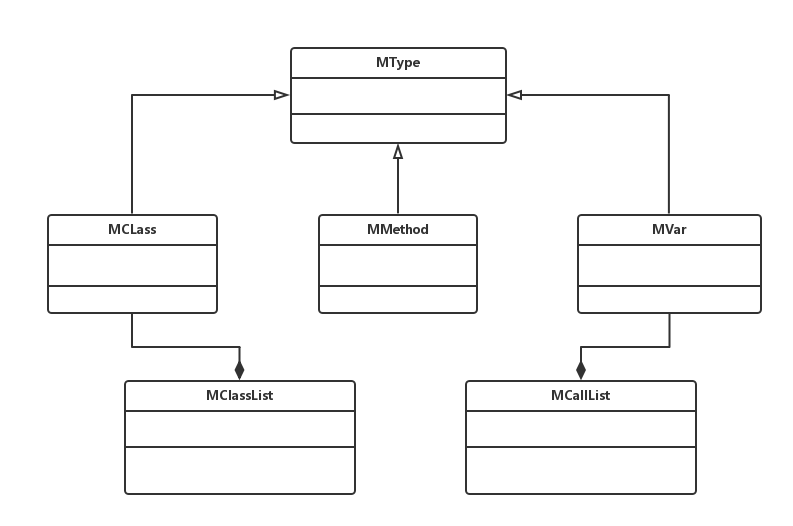
\includegraphics[height=170pt]{4.png}
	\item类图说明
	\end{enumerate}
	\paragraph{}
	\begin{table}[!hbp]
	\begin{tabular}{c|c}
	\hline
	类名 & 说明 \\
	\hline
	MClassList & 全局只有一个对象,记录一个minijava程序中所有出现的类 \\
	\hline
	MType & MClass,MMethod,MVar等类的父类 \\
	\hline
	MClass & 每一个类对应一个MClass对象 \\
	\hline
	MMethod & 每一个方法对应一个MMethod对象 \\
	\hline
	MVar & 每一个变量对应一个MVar对象 \\
	\hline
	MCallList & 一次函数调用会生成一个MClassList对象,存储参数列表 \\
	\hline
	\end{tabular}
	\end{table}
	每个类的核心成员如下:
	\begin{enumerate}
	\item MClassList类:
	\begin{lstlisting}[language=Java]
public class MClassList {
	private ArrayList<MClass> mClassArrayList;
}
	\end{lstlisting}
	\item MType类:
	\begin{lstlisting}[language=Java]
public class MType {
	private String name;
	private int line;
	private int column;
}
	\end{lstlisting}
	\item MClass类:
	\begin{lstlisting}[language=Java]
public class MClass extends MType {
	private ArrayList<MMethod> mMethodArrayList;
	private ArrayList<MVar> mVarArrayList;
	private String parentClass;
} 
	\end{lstlisting}
	\item MMethod类:
	\begin{lstlisting}[language=Java]
public class MMethod extends MType {
	private String returnType;
	private String className;
	private ArrayList<MVar> mParamArrayList;
	private ArrayList<MVar> mVarArrayList;
}
	\end{lstlisting}
	\item MVar类:
	\begin{lstlisting}[language=Java]
public class MVar extends MType {
	private String type;
	private String isParam;
	private String methodName;
	private String className;
}
	\end{lstlisting}
	\item MCallList类:
	\begin{lstlisting}[language=Java]
public class MCallList extends MType {
	private MMethod callerMethod;
	private MMethod calleeMethod;
	private ArrayList<MVar> mVarArrayList;
}
	\end{lstlisting}
	\end{enumerate}
	\subsubsection{注意点}
	\paragraph{}
	\begin{enumerate}
	\item子类对象可以赋值给对象,所以在判断类型是否一致时,不能简单判断两者类型是否完全一样
	\item判断完循环继承后,建议切断循环圈中任一一个继承关系,以防止后面的代码陷入死循环
	\item minijava支持方法的覆盖,但是不支持重载.判断一个方法和父类的同名方法是重载还是覆盖比较考验细心.调用一个子类对象的覆盖过后的方法时,应当是调用子类的同名方法.但子类对象也应当能找到父类中的方法,我的做法是,先为父类,子类各自建立类声明时定义的方法,在第一遍语法树遍历完成之后,把父类中的方法都添加给子类,此时,父类被覆盖的方法就不再添加了.
	\end{enumerate}
	
	\subsection{中间代码生成}
	\subsubsection{阶段目标}
	\paragraph{}
	中间代码生成阶段的目标是将minijava源代码转换成中间代码Piglet.Piglet与minijava的区别主要如下:
	\begin{enumerate}
	\item采用前缀表达式
	\item引入了临时单元
	\item函数的参数个数限制为20个
	\item分支与循环需要变成标签和跳转
	\item需要考虑内存分配和管理
	\end{enumerate}
	\subsubsection{代码说明}
	\paragraph{}
	本阶段包含的代码有:
	\begin{enumerate}
	\item包minijava.minijava2piglet
	\item类minijava.visitor.SymbolTableVisitor
	\item类minijava.visitor.MinijavaToPigletVisitor
	\end{enumerate}
	\subsubsection{方法概述}
	\begin{enumerate}
	\item扩展原有的符号表,在原先符号表的元素基础上,扩展如下:
	\paragraph{}
	\begin{lstlisting}[language=Java]
public class MType {
	private int tempNum; 
		// Temp unit correspond to a parameter or a varaiable
	private int offset; 
		// Offset for a variable or a method inside a class
} 

public class MMethod {
	private String pigletName; 
		// Label name for a method
}
	\end{lstlisting}
	\item使用类型检查步骤中的SymbolTableVisitor遍历语法树,建立符号表
	\item建立每个类的存储模型,变量/方法需记录offset,同时方法记录piglet中对应的标签名,把方法参数和0-19号寄存器关联起来
	\item用MinijavaToPigletVisitor遍历语法树,翻译成Piglet代码
	\end{enumerate}
	\subsubsection{类的存储结构}
	\begin{enumerate}
	\item{结构图}
	\paragraph{}
	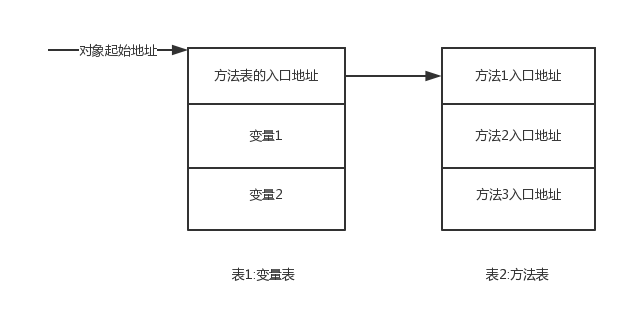
\includegraphics[height=200pt]{2.png}
	\item{结构图说明}
	\end{enumerate}
	\paragraph{}
	从minijava翻译到piglet,最重要的就是把变量/方法地址和临时单元联系起来.一个类实例化时,需要为它分配空间.我的存储办法是一个对象有两个表,上图中的表1存储变量(基本类型,如Integer,Boolean就直接存储值,对于复合类型,存储首地址),表2存储方法的入口地址,由minijava的性质保证:两个表中每个元素都是4字节.为了方便的由一个类的起始地址找到两个表,表1的前4个字节存储表2的起始地址.
	\subsubsection{注意点}
	\begin{enumerate}
	\item由于minijava中不同的类可以有相同的方法名,转换到piglet中的方法的标签时,为了防止冲突,我采用"类名+下划线+方法名"的办法加以区分
	\item对于对象的方法表,上图中的表2,节省空间的做法是相同类的所有对象存储一张表.我的做法是为每一个对象生成一个方法表,这样编写代码比较方便
	\item对于继承,我采用了和类型检查时类似的方法.在遍历语法树翻译之前,我就为每个类增加了父类的方法和变量.对于覆盖的方法,是不需要添加的
	\item比较麻烦的是调用方法节点的翻译,需要先找到这个实例的首地址,再根据方法的偏移量到方法表中去找对应的方法入口地址
	\item数组的处理,我采用了比较普遍的方法,对于一个长度为L的数组,分配L+1个字节的存储空间,第一个字节存储数组长度L,之后依次存储数组的内容
	\item对于多于20个参数的方法调用,本编译器并未做处理
	\end{enumerate}
	\subsection{中间代码简化}
	\subsubsection{阶段目标}
	\paragraph{}
	中间代码简化阶段的目标是生成更接近汇编代码的中间代码Spiglet.主要需要在Piglet的基础上做一下两种变化:
	\begin{enumerate}
	\item不允许嵌套表达式
	\item表达式只允许出现在MOVE中
	\end{enumerate}
	\subsubsection{代码说明}
	\paragraph{}
	本阶段包含的代码有:
	\begin{enumerate}
	\item包piglet.piglet2spiglet
	\item类piglet.visitor.PigletTempNumVisitor
	\item类piglet.visitor.Piglet2SpigletVisitor
	\end{enumerate}
	\subsubsection{方法概述}
	\paragraph{}
	\begin{enumerate}
	\item遍历一遍语法树,统计原先Piglet使用了多少个临时单元
	\item以上的临时单元全部保留,遇到复合表达式时,新申请一个临时单元,把表达式的结果保存到这个临时单元中,返回这个临时单元
	\end{enumerate}
	\subsubsection{注意点}
	\paragraph{}
	这一步相对简单,也可以从minijava直接翻译成spiglet.这里就上述步骤2举一个实际翻译的例子:
	\begin{lstlisting}[language=Java]
	/**
	 * f0 -> Operator()
	 * f1 -> Exp()
	 * f2 -> Exp()
	 */
	public MSpiglet visit(BinOp n) {
		/* MSpiglet is a new data structure defined by me.
		 * It contains the Spiglet code generated by each node.
		 * Each node returns a MSpiglet object.
		 */
		MSpiglet _ret = new MSpiglet("");
		MSPiglet op = n.f0.accept(this);
		MSpiglet exp1 = n.f1.accept(this);
		MSpiglet exp2 = n.f2.accept(this);
		_ret.appendCode(exp1);
		_ret.appendCode(exp2);
		String name = getNextTemp();
		_ret.appendCode(new MSpiglet("MOVE " + name + " " 
		+ op.getOp() + " " + exp1.getTemp() + " " + exp2.getTemp()));
		// Move result to a new temp unit
		_ret.setTemp(name);
		return _ret;
	}
	\end{lstlisting}
	\subsection{寄存器分配}
	\subsubsection{阶段目标}
	把Spiglet代码翻译成对应的Kanga代码,主要有以下几方面的挑战:
	\begin{enumerate}
	\item标号改为全局
	\item几乎无限的临时单元改为有限的寄存器,具体的寄存器情况如下:
	\begin{enumerate}
	\item a0-a3:存放向子函数传递的参数
	\item v0-v1:v0存放子函数返回结果,v0,v1还可以用于表达式的求值
	\item s0-s7:存放局部变量,在发生函数调用时要保存
	\item t0-t9:存放临时运算结果,在发生函数调用时不需要保存
	\end{enumerate}
	\item引入栈.有专门的指令用于从栈中加载(ALOAD),向栈中存储(ASTORE),SPILLEDARG i代表栈中的第i个值
	\item不再使用函数调用语句传递参数,需要把参数和运算结果放在对应寄存器中完成传递
	\item过程的头部包含3个整数(如:proc[5][3][4])
	\begin{enumerate}
	\item第一个整数表示参数个数
	\item第二个整数表示过程中需要的栈单元个数,包含参数,溢出单元,需要保存的寄存器
	\item第三个整数是procA过程中最大的参数数目.例如,procA调用procB用3个参数,调用procC用2个参数,那么这么整数设为3
	\end{enumerate}
	\end{enumerate}
	\subsubsection{代码说明}
	\paragraph{}
	本阶段用到如下代码:
	\begin{enumerate}
	\item包spiglet.spiglet2kanga
	\item类spiglet.visitor.LivenessAnalysisVisitor
	\item类spiglet.visitor.Spiglet2KangaVisitor
	\end{enumerate}
	\subsubsection{方法概述}
	\begin{enumerate}
	\item遍历语法树,活性分析,为每个statement记录关联的临时单元,下一条statement,当前标签,如果是跳转,还要记录跳转至的标签
	\item寄存器分配,确定溢出临时单元在栈中的位置(spilledarg后的参数)
	\item再次遍历语法树,完成翻译
	\end{enumerate}
    \subsubsection{本阶段数据结构与算法设计}
    \begin{enumerate}
    \item活性分析:这一阶段我为每一个statement建立一个SStat对象,记录出现的临时单元(记录在usedTempList中),跳转信息.为之后建立干扰图,图染色算法做准备
    \begin{lstlisting}[language=Java]
public class SStat {
    public ArrayList<Integer> usedTempList;  
        // Temp units used by the statement
    public String jumpLabel,entryLabel;
    public boolean isUnconditionalJump;
    public SStat nextStmt1,nextStmt2;
        // nextStmt1 is statement follows right after this statement,
        // nextStmt2 is statement is statement when jump happens
    public HashSet<Integer> outSet; 
        // Temp units alive in this statement
}
    \end{lstlisting}
    \item建立干扰图:
    \begin{enumerate}
    \item根据statement的entryLabel域把代码分块
    \item根据statement的isUnconditional域和jmupLabel域,填nextStmt1域(紧邻的下一句)和nextStmt2域(跳转到标签的第一句)
    \item迭代更新每条语句里活跃的临时单元(除了这句中直接用到的,还有它所处块之后的语句中用到的单元),直到不发生变化。最终结果记录在SStmt的outSet域
    \end{enumerate}
    \item图染色算法:
    干扰图建立完毕后开始着色,图着色算法每次挑选干扰图中度数最大且还未染色的点,将与其相邻的已染色的点的颜色编号保存在一个集合中。最后找到最小的不在集合中的颜色编号并分配给该点。
    \item建立起临时单元和寄存器或栈空间的映射关系,因为寄存器的环境更改以方法调用为界限,我为每个方法定义了如下数据结构,其中图染色的结果保存在regForTemp中:
    \begin{lstlisting}[language=Java]
public class SMethod {
    public String name;
        // Method name
    protected ArrayList<SStat> statArrayList;
        // Statements inside this method
    protected HashSet<Integer> tempSet;
        // All temp units used in the method
    protected TreeMap<Integer,Integer> regForTemp;
        // Mapping between register number and temp unit id
    public int paramNum,spilledNum,spilledSize;
        // spilledNum: number of spilled args; 
        //spilledSize: number of spilled local variables
}
    \end{lstlisting}
    \end{enumerate}
    \subsubsection{注意点}
    \paragraph{}
    这一节列举一些翻译时要注意的地方
    \begin{enumerate}
    \item进入函数之前,要把s0,s1...s7压栈保存
    \item从栈中读数保存到寄存器时,可以用v0,v1进行中转
    \item Kanga函数头部第一个参数比较容易,第三个参数我之前就没有对20个参数以上的情况作处理,所以我设定的是20.第二个参数我的算法是用SMethod中的spilledNum和spilledSize相加,前者是溢出的参数个数,后者是溢出的局部变量个数.栈中的存储关系是SPILLEDARG 0-(spilledNum-1)存储溢出参数,变量接在后面存储
    \end{enumerate}
    \subsection{目标代码生成}
    \subsubsection{阶段目标}
    \paragraph{}
    这阶段的任务是把kanga代码转为mips代码。主要区别是:
    \begin{enumerate}
    \item需要手动管理栈指针和帧指针
    \item涉及系统调用
    \end{enumerate}
    \subsubsection{代码说明}
    本阶段的代码包括:
    \begin{enumerate}
    \item包kanga.kanga2mips
    \item类kanga.visitor.Kanga2MipsVisitor
    \end{enumerate}
    \subsubsection{方法概述}
    \begin{enumerate}
    \item遍历语法树,翻译对应的mips代码
    \end{enumerate}
    \subsubsection{mips栈结构}
    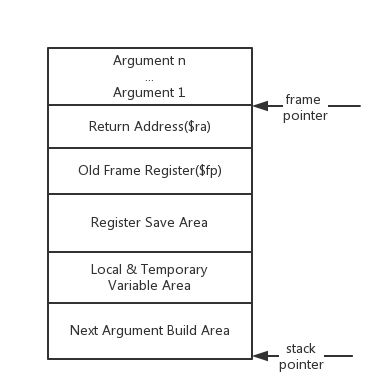
\includegraphics[height=300pt]{3.png}
    \subsubsection{注意点}
    \begin{enumerate}
    \item在调用一个函数时,需要:
    \begin{enumerate}
    \item保存老的帧指针和返回地址
    \item把原先的栈指针的值赋给帧指针
    \item根据kanga函数头指定的需要栈单元个数分配足够的栈空间
    \end{enumerate}
    \item在函数返回时,需要恢复现场,回收栈空间,最后跳转到返回地址指定的位置
    \item对Kanga中的Exp()节点处理时,需要分别对IntegerLiteral,Label,Reg三种情况处理
    \end{enumerate}
\section{测试与调试}
    1.类型检查测试用例:\\
    提供的有脚本测试的100个测试用例基本上只包含一个,最多两个错误。而类型检查的一大难点是多个错误混合嵌套。在这种情况下即使不要求检查出所有错误,但要求保证程序的稳定性也有一定的困难。\\
    一些比较容易出错的情况有:
    \begin{enumerate}
    \item循环即成与覆盖同时出现
    \item类重定义时,后定义的类引用前一个类的变量
    \end{enumerate}
    2.各步翻译:除了教学网提供的4个例子,在UCLA的网站上,共有8个例子可供测试。我每一步的翻译后的测试都是用解释器检查这8个例子是否正确
\section{实习总结}
    \paragraph{}
    \indent\indent结束了一个学期的编译实习工程,写完之后还是很有成就感的。就一门课而言,这门课要花费的时间和精力确实比较多。整个项目完成,我对编译的整个过程有了更深的了解,虽然词法分析和语法分析部分都是直接套用了现有的工具,但通过课程开始的入门调研,对jtb和javacc这些工具也有了一定的了解。\\
    \indent\indent要说最大的收获,我觉得是visitor模式的学习和使用。这是一种很好的设计模式,很好的分离了类和操作。将不同类的相同操作汇总在一个visitor中,用visitor中函数的重载替换类的多态。要为一个类增加操作的时候,通常的设计方法是父类增加一个抽象方法,所有子类各自实现各自的方法,这样以来需要修改所有的子类。而采用visitor模式,只需要新设计一个visitor,在该visitor中实现不同的操作即可。
\end{spacing}
\end{CJK}
\end{document}  
